
\documentclass[12pt]{article}

\usepackage[T1]{fontenc}
\usepackage[version=4,arrows=pgf-filled,
textfontname=sffamily,
mathfontname=mathsf]{mhchem}
\usepackage[utf8]{inputenc}
\usepackage{svg}
\usepackage{lmodern}
\usepackage{bm}
\usepackage{gensymb}
%\usepackage{subcaption}
\usepackage{amsmath,amssymb}
\usepackage{braket}
\usepackage{booktabs}
\usepackage{multirow}
\usepackage[english]{babel}
\usepackage{csquotes}
\usepackage[document]{ragged2e}
\usepackage{amsmath}
\usepackage{tikz, pgfplots}
\usepackage{romannum}
\usetikzlibrary{shapes.geometric}
\usetikzlibrary{positioning}
\usetikzlibrary{matrix,decorations.pathreplacing, calc, positioning,fit}
\usetikzlibrary{arrows}
\usepackage[labelfont=bf]{caption}
\usepackage{graphicx}
\usepackage{tikz}
\usepackage{tkz-euclide}
\usepackage{tikz-cd}
\usepackage{pgfplots}
\usepackage{pgf}
\usepackage{lmodern}
\usepackage{import}
\pgfplotsset{width=1cm, compat=1.9}
\usepackage{tikz,venndiagram}
\usepackage{subfig}
\usepackage{centernot}
\usepackage{mathtools}
\usepackage{hyperref}
\usepackage{float}
\vspace{-5pt}
\hypersetup{
    colorlinks=true,
    linkcolor=blue,
    pdftitle={Overleaf Example},
    pdfpagemode=FullScreen,
    }
\usepackage[sorting=none]{biblatex}
\addbibresource{bib.bib}
\AtBeginDocument{\pagenumbering{arabic}}

\usepackage{cleveref}

\begin{document}
\pagenumbering{gobble}
\begin{center}
\huge{Freie Universität Berlin}\\[10pt]
\huge{Advanced Laboratory Course}\\[50pt]
\huge{\textbf{Auger and Electron Energy Loss Spectroscopy (Ma10)}}\\[60pt]
\large{Rocky Kamen-Rubio and Federico Porcelli (Group M9)}\\[30pt]
\large{Supervisor: Dr. Md Sabbir Ahsan}\\[30pt]
\large{Experiment conducted on 31.10.2024}\\[30pt]
\end{center}

\begin{abstract}
\justifying Auger electron spectroscopy (AES) and Electron Energy Loss Spectroscopy (EELS) are important surface analysis tools that allow for investigating the electronic structure and chemical composition of material surfaces. These spectroscopic techniques have been applied to investigate solid aluminum. The dataset was collected using a laboratory Auger spectrometer and an EELS analyzer, with lock-in amplification based cylindrical mirror analyzer, enabling the identification of core-level shifts, plasmon excitations, and electronic transitions.
\end{abstract}

%\begin{abstract}
%\justifying This experiment focuses on Auger electron spectroscopy (AES) and Electron Energy Loss Spectroscopy (EELS). By recording the first derivative spectrum of the energy distribution of electrons \( \frac{dN(E)}{dE} \), we analyzed how the number of detected electrons varies with their energy. From this spectrum, we recognized both the Auger processes and the creation of bulk and surface plasmons, correctly matching the theoretical expectations.
%These techniques allow for investigating the electronic structure and chemical composition of material surfaces. The dataset was collected using a laboratory Auger spectrometer and an EELS analyzer, enabling the identification of core-level shifts, plasmon excitations, and electronic transitions.
%\end{abstract}



\tableofcontents

\pagenumbering{arabic}
\section{Introduction}
\rule{\textwidth}{0.5pt}
\justifying
Spectroscopy, specifically Auger electron spectroscopy (AES) and electron energy loss spectroscopy (EELS), are powerful methods for studying the interaction of electrons with the surface of materials. These techniques provide detailed information about surface composition and electronic structure, making them essential in materials science and surface physics. AES relies on the detection of Auger electrons emitted when an atom’s inner-shell electron is ejected, causing a cascade effect where another electron is emitted. The energy of this emitted electron depends on the electronic structure of the atom and can be used to identify the elemental composition of the sample’s surface. The energy of these Auger electrons is characteristic of the element, providing a non-destructive way of identifying the atomic composition of a material’s surface. EELS, on the other hand, measures the energy lost by electrons as they pass through or reflect off a material. This energy loss occurs due to inelastic scattering, where electrons interact with the atoms in the material, revealing information about electronic excitations, such as plasmon resonances and band structure. Together, AES and EELS offer complementary information about the surface properties and electronic behavior of materials.

% \newpage
\subsection{Theoretical background}

%\subsubsection{Auger electron spectroscopy (AES)}
Figure \ref{fig:auger} illustrates the two main steps that characterize the Auger process. Namely, starting from an atom from which an electron in the 1s state has been removed (ionization), an outer electron fills the core hole and transmits the available energy to a second electron which leaves the atom.

The Auger transition is notated with 3 letters ($K, L, M, ...$ for the quantum numbers $n=1, 2, 3, ...$) to represent the three electron states. In particular the first letter comes from the shell of the initial hole (K), the second letter from the electron which fills this hole, and the third from the kicked out electron. Thus, a $\text{K}_1\text{L}_1\text{L}_{2,3}$ transition means that starting from an inital missing electron in the 1s orbital, an electron from the 2s state fills this void, and one from the 2p state is emitted. Note that the energy of the emitted electron is the same regardless of the order of the states, but by convention we write the highest energy state last.

The Al-KLL transition energies are reported in Table \ref{tab:transition}. However, the intensity of the peaks is not equal, and depends on the amount of electrons available for that transition to occur.

As Figure \ref{fig:transitions} shows, the most intense peaks are, from strongest to least strong, $\text{KL}_{2,3}\text{L}_{2,3}\ ({}^1D)$, $\text{KL}_{1}\text{L}_{2,3}\ ({}^1P)$, $\text{KL}_{1}\text{L}_{2,3}\ ({}^3P)$, $\text{KL}_{2,3}\text{L}_{2,3}\ ({}^1S)$ and $\text{KL}_{1}\text{L}_{1}\ ({}^1S)$.
\begin{figure}[H]
  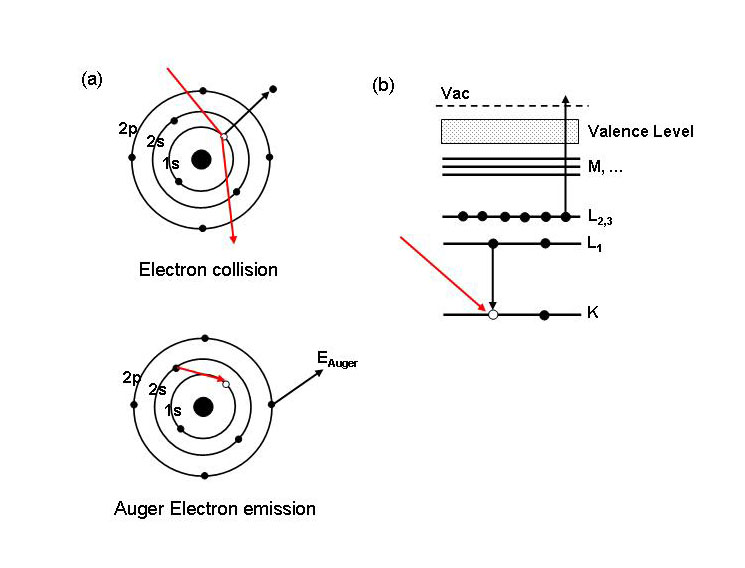
\includegraphics[width=\linewidth]{Auger_Process.jpg}
  \caption{Auger process schematized in two steps, and X-Ray notation drawing, taken from Wikipedia \cite{wiki:auger}}
  \label{fig:auger}
\end{figure}

\begin{figure}[h!]
  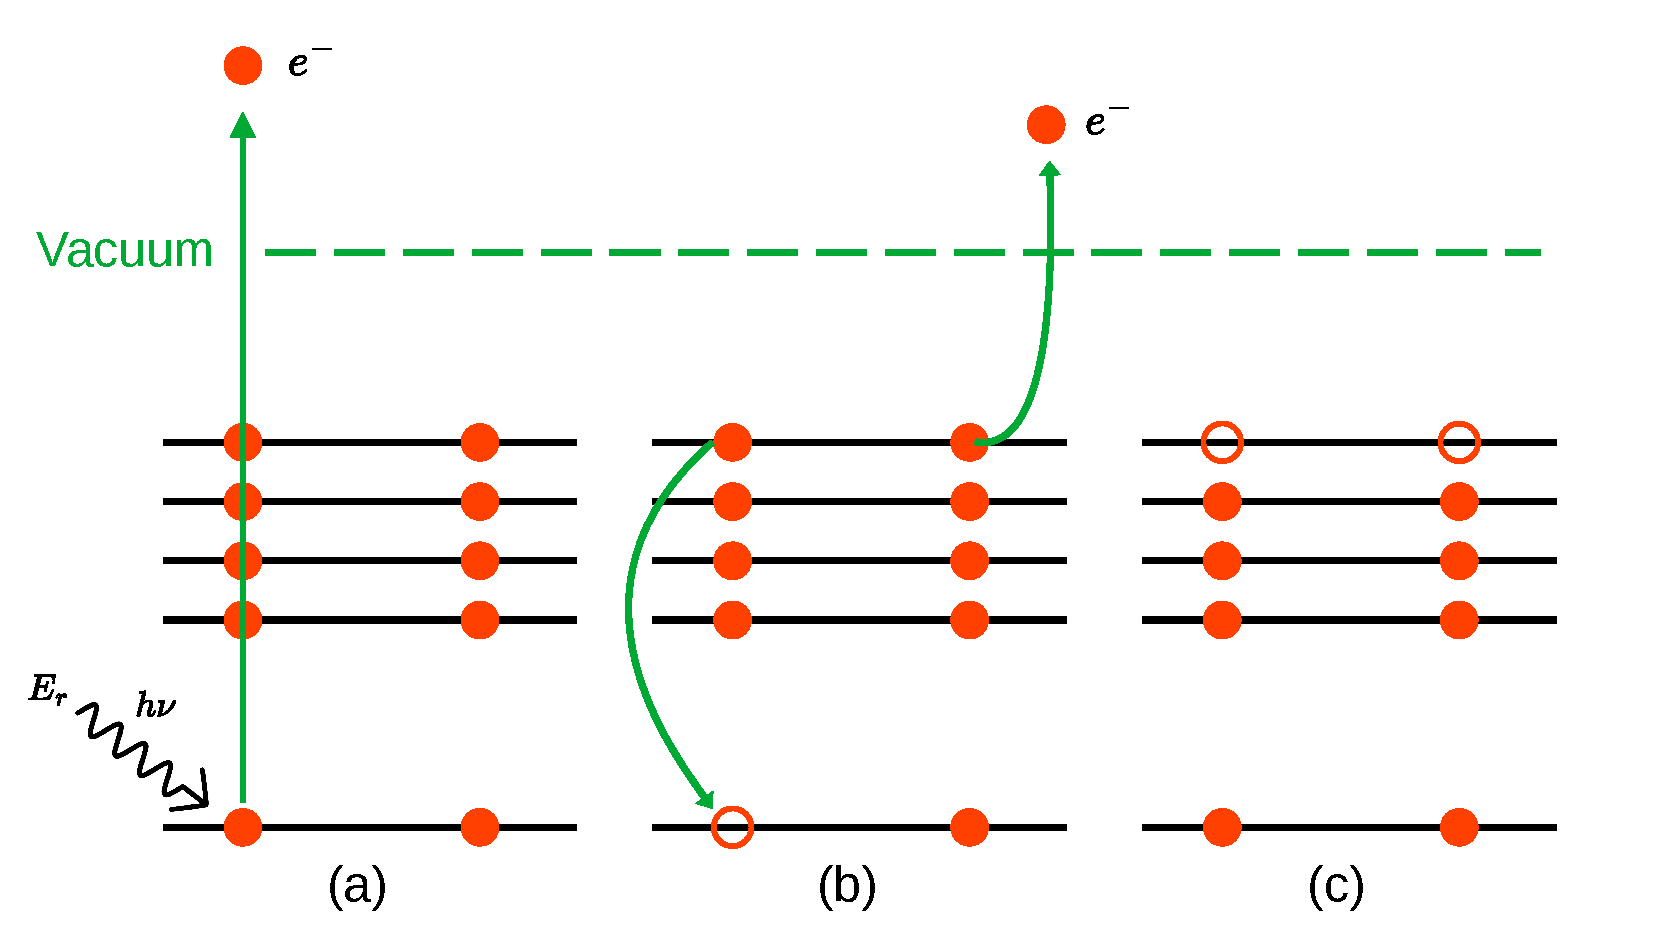
\includegraphics[width=\linewidth]{sabbirdrawing.pdf}
  \caption{The three steps involved in the Auger process. First, an electron in the lowest energy state (1s) is excited by a photon (a). The gap is then filled by an electron in one of the higher energy states, and by conservation of momentum, another electron is emitted (b). The resulting electron configuration is thus missing two electrons in comparison to the initial state (c).}
  \label{sabbirdrawing}
\end{figure}


% \subsubsection{Highest intensity peaks in Al-KLL-spectrum}

\begin{figure}
  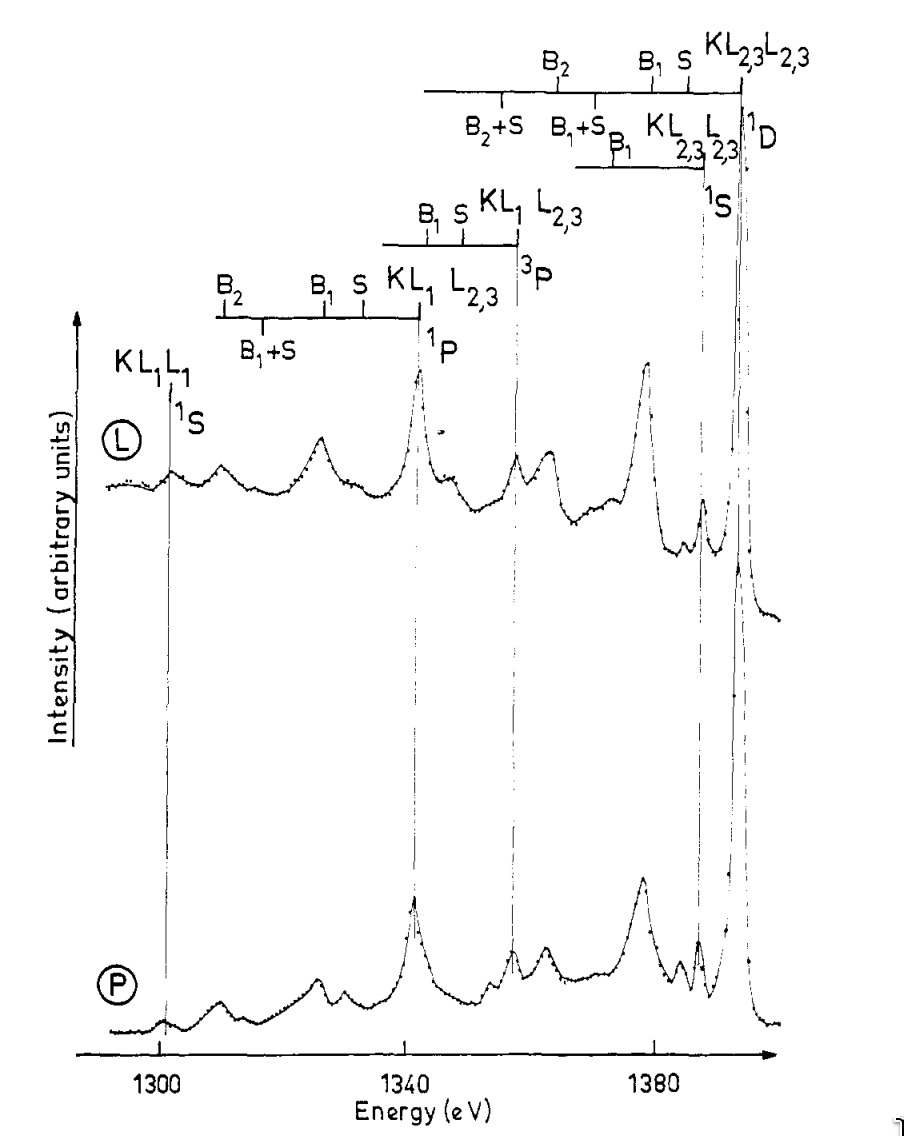
\includegraphics[width=\linewidth]{augerspectrumal.png}
  \caption{Electron induced Auger-KLL spectrum of Aluminum, taken from \cite{dufor}}
  \label{fig:transitions}
\end{figure}

\begin{table}[h!]
    \centering
    \begin{tabular}{lcc}
        \toprule
        \textbf{Auger line} & \textbf{E(lab) (eV)} & \textbf{E(theory) (eV)} \\
        \midrule
        K-L$_{2,3}$L$_{2,3}$ ($^{3}$P) & Not obs. & (1398.1) \\
	K-L$_{2,3}$L$_{2,3}$ ($^{1}$D) & 1393.1 & 1393.5 \\
        K-L$_{2,3}$L$_{2,3}$ ($^{1}$S) & 1387.1 & 1386.6 \\
        K-L$_{1}$L$_{2,3}$ ($^{3}$P) & 1357.2 & 1358.5 \\
        K-L$_{1}$L$_{2,3}$ ($^{1}$P) & 1341.6 & 1342.3 \\
        K-L$_{1}$L$_{1}$ ($^{1}$S) & 1302.6 & 1304.0 \\
        \bottomrule
    \end{tabular}
    \caption{Energy values for different Auger lines. Taken from \cite{fu2024auger}.}
    \label{tab:transition}
\end{table}

\subsubsection{Plasmons}

Metals have a highly delocalized outer shell of electrons which, when perturbed by an incident particle like an electron, can create quasiparticle oscillations called plasmons. We call such oscillations in the bulk of a solid bulk plasmons, and those at the interface between a metal and a dialectric surface plasmons. Surface plasmons generally have lower energy, because of the different boundary conditions and confinement effects. In the case of bulk plasmons, the oscillations occur throughout the volume of the material, whereas surface plasmons are confined to the interface, leading to a lower restoring force and hence a lower resonant energy.
\subsubsection{Bulk/surface plasmon observations}

In aluminum, the bulk plasmon excitation energy is approximately 15.2 eV, and the surface plasmon excitation energy is about 10.4 eV. However, in practice, much higher energies—around 1000 eV for bulk plasmons and 200 eV for surface plasmons—are supplied to observe these excitations. This discrepancy arises due to the influence of the universal mean free path of electrons, which governs how far electrons can travel through the material without significant scattering. Higher incident electron energies are necessary to overcome these constraints and ensure the effective excitation and detection of plasmons in different regions of the material.
\subsubsection{Universal Mean Free Path }
\begin{figure}[H]
  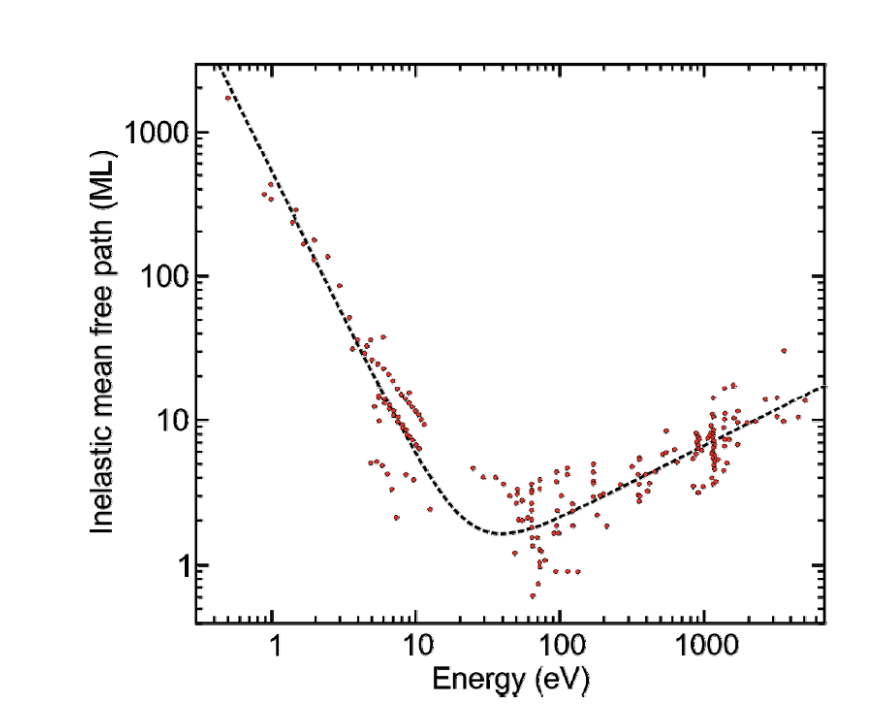
\includegraphics[scale=0.7]{Universal_mean_free_path.png}
  \caption{Universal curve of the inelastic mean free path of electrons in elements given in atomic monolayers, taken from \cite{seah1979quantitative}}
  \label{fig:mfp}
\end{figure}
The Universal Mean Free Path corresponds to the relationship between electron kinetic energy and the inelastic mean free path, indicating the surface vs bulk sensitivity, as well as the probe depth. For incident electrons with $10^3eV$ kinetic energy, we anticipate a probe depth of $10-30\AA$. The full reference curve is shown below (Figure \ref{fig:mfp}).

AES is highly surface-sensitive, as the emitted electrons come from the outermost atomic layers, typically 1-10 nm in depth.

\subsubsection{Electron Energy Loss Spectroscopy (EELS)}
EELS involves the inelastic scattering of electrons as they pass through or are reflected from a material. The energy lost by the electrons during this process provides valuable information on the material's electronic structure. Peaks in the EELS spectrum can correspond to various electronic excitations, including interband transitions and plasmon excitations, which give insight into the material's dielectric function and electronic behavior. We expect to see the possible Auger transitions, and satellite peaks that are a unit of plasmon energy away from the main Auger peaks.

%(ADD AND EXPLAIN DIAGRAMS!)

% \newpage
\subsection{Experimental setup}

% \subsubsection{CMA with integrated electron gun}
The cylindrical mirror analyzer (CMA) is used to energetically filter the emitted or scattered electrons. It consists of two conducting coaxial cylinders with a potential gradient across them. When the electrons enter the generated electric field, their trajectories curve based on their incident kinetic energy. The potential difference between the cylinders creates an electric field that selectively allows electrons of certain energies to pass through an exit slit, which can be adjusted to vary the range of kinetic energies being analyzed (Figure \ref{fig:cma}).

% \subsubsection{Generation and acceleration of free electrons}
An integrated electron gun (thermoionic cathode) is used to fire incident electrons at the sample. This gun heats a anodic piece of metal (usually and in this case Tungsten) that emits electrons via thermionic emission. They then are accelerated through an electric field generated between the emitting anode and cathode farther down the barrel of the gun. The power supply for the electron gun provides the current for the thermionic cathode (where electrons are generated via thermionic emission) and the acceleration (up to 5 kV!), focusing, and deflection voltages.


\begin{figure}[!h]
    \centering
    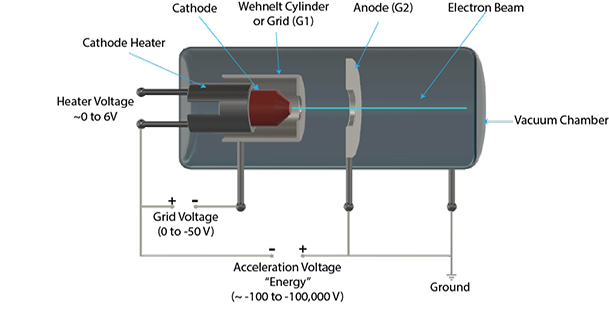
\includegraphics[width=0.75\textwidth]{Electron_Gun_simple_schematic_20190402v1-crop-u11694.png} % Replace 'example-image' with your image file name
     \caption{Schematic of a thermionic cathode electron gun \cite{jeol2012thermionic}}
    \label{fig:example}
\end{figure}


% \subsubsection{CMA energy filtering}
The CMA filters electrons based on their kinetic energy by exploiting the relationship between the electric field and the electron’s energy-dependent curvature (Figure \ref{fig:cma}). By varying the voltage applied to the outer cylinder, the potential gradient is changed, and therefore the range of energies that can successfully pass through the exit slit to reach the detector. Thus, a precise selection of the desired energy band can be achieved.

% \subsubsection{Ulta-High Vaccum (UHV)}

In this experiment, an ultrahigh vacuum (UHV) chamber (lower than $10^{-9}$ torr) will be used. This is important because even a small amount of oxygen or water can contaminate the surface of our sample and influence our results. Since we are only measuring a few angstroms deep, it is important for our sample surface to be clean. Furthermore, if the vacuum isn't strong enough, electrons emitted from the sample could interact with gas particles in the chamber, affecting our reading.

The UHV chamber is also equipped with a cylindrical mirror analyzer (CMA) for the AES and EELS experiments. The vacuum is generated by a combined system of turbomolecular and membrane pumps as well as an ion getter pump. The pressure is measured with a cold cathode ionization gauge.


\subsubsection{Lock-In amplifier and signal amplification}
A lock-in amplifier is used to improve the signal-to-noise ratio. Lock-in amplifiers rely on phase-sensitive detection, which demodulates or rectifies an AC signal using a reference waveform derived from the source that modulated the signal. This means that the lock-in amplifier will respond primarily to signals that are coherent (having the same frequency and phase) with the reference waveform while rejecting all other signals.

The operation of the lock-in amplifier is particularly useful in environments where the signal is weak compared to noise. In the context of our experiment, we are interested in recording a first derivative spectrum of the energy distribution of the electrons, represented by \( \frac{dN(E)}{dE} \), as derivative Gaussian's yield better fits and will give a clearer peak at the 0-crossing.

The oscillating signal arises from the modulation of the electron beam or the excitation of the sample, and measuring \( \frac{dN(E)}{dE} \) allows us to analyze how the number of detected electrons varies with their energy.


%    \item A channeltron to detect the electrons after they have been filtered by energy. It operates with high voltage (up to 3 kV) and is a continuous version of a dynode-channel type secondary-electron multiplier. This means that the channeltron uses a series of dynodes to amplify the current generated by the incident electrons. When an electron strikes the channeltron's inner surface, it emits secondary electrons, which are then accelerated towards the next dynode, causing further emission. This cascading effect allows for significant amplification of the detected signal.


\begin{figure}
  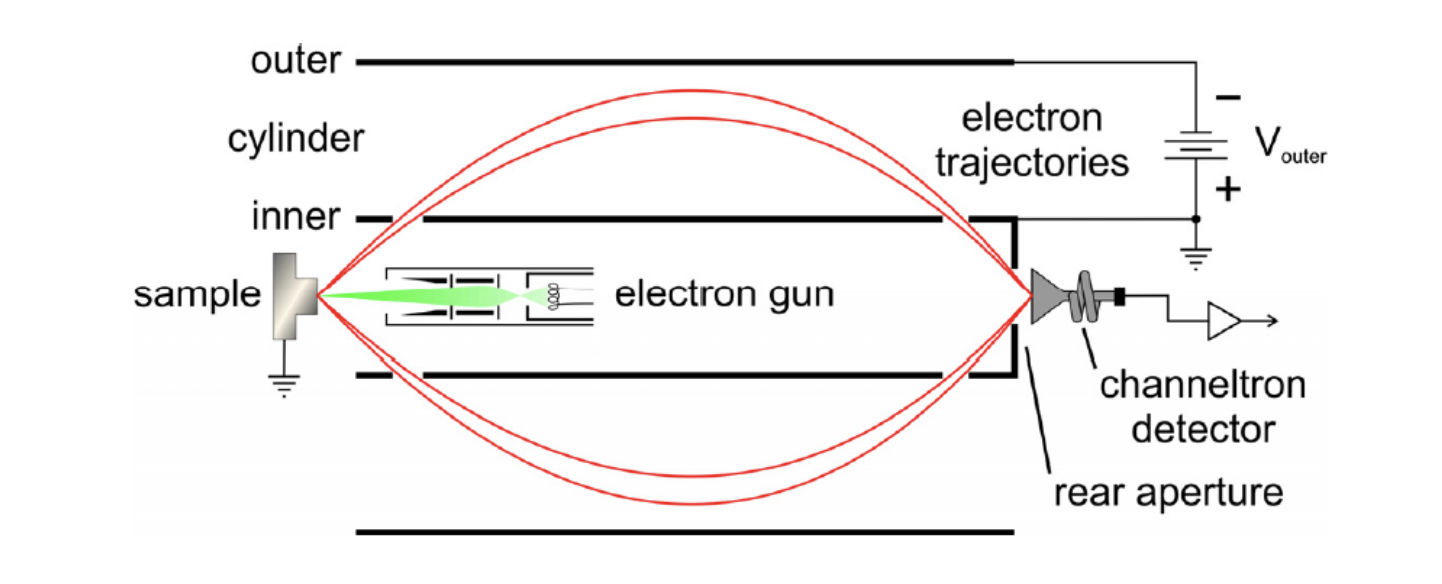
\includegraphics[width=\linewidth]{setup_schematic.png}
  \caption{Schematic cross section view of a cylindrical mirror analyzer (CMA) with an integrated electron gun (taken from \cite{fu2024auger}).}
  \label{fig:cma}
\end{figure}

% \newpage
\section{Results and Discussion}
\subsection{Uncleaned Al sample}
As a first measurement, we focused on the uncleaned sample of Aluminum. After having checked that the chamber was correctly evacuated (at a pressure of $3.5 \times 10^{-9}\text{ mbar}$), we turned on the switches for both the power supply of the electron gun and the CMA. Then, we slowly raised the voltage of the electron gun to about 100eV, and raised the current until about 1.9 A. Only then did we increase the voltage to 4000 eV, so as to prevent any possible damage to the wire by overly quick voltage changes.

The reason for choosing the filament energy arises from two considerations. In the first place, the 1s ionization threshold of the Aluminum being 1558.20 eV \cite{palmberg1991handbook} means that we need to provide a filament energy that is above this threshold, otherwise the 1s-ionization cannot occur. Secondly, we want to maximize the scattering cross section of the emitted Auger electrons, so that as many of them can be detected by the CMA. In general, the greatest cross section is obtained when the supplied energy is about three times as big as the ionization energy of the sample. In the case of aluminum, then, it would amount to $3 \cdot 1558 \text{ eV}\approx 4600 \text{ eV}$. Therefore, choosing our filament energy to be 4000 eV maximizes the cross section, while still limiting the filament wear.

Then the CMA voltage was set to 1.8kV, and a spectrum was recorded with a phase of 156\degree, a sensitivity of $300 \mu $V, a time constant of 300 ms, and the oscillator level of 1.5 V (Figure \ref{uncleaned}).


Derivatives of Gaussian functions, i.e. \[
G'(x) = -\frac{(x - \mu)}{\sigma^3 \sqrt{2 \pi}} e^{-\frac{(x - \mu)^2}{2 \sigma^2}}
\]  were then used to fit the most intense transitions in the spectrum, which correspond, respectively, to the Aluminum $\text{L}_{2,3}\text{VV}$, the Carbon and Oxygen KVV and the Al $\text{KL}_{2,3}\text{L}_{2,3}$ transitions. In the formula, $x$ represents the energy (independent variable), $\mu$ the peak position (i.e. point where the derivative is zero), and $\sigma$ the width of the peak.
This was done to extrapolate the correct energy at which each transition occurs (i.e. $\mu$). These values are reported in Table \ref{tab:alpeaks}, and compared to the NIST experimental predictions.


\subsection{Cleaned Al sample}
The CMA and electron gun were then turned off, and the surface of the sample was cleaned using an abrasive metal brush, all the while inside the vacuum. Proper attention was given to make sure that the vertical position of the sample remained unchanged, so as to prevent possible changes in the measured area and thus in the spectrum.
After turning on the instrumentation again, a measurement was performed in a similar fashion as for the uncleaned aluminum. In particular, we ensured that the parameters of sensitivity, phase etc. remained unchanged, so as to isolate the difference between cleaned and uncleaned sample.

Two of the main peaks have disappeared (mostly) in the resulting spectrum - those due to carbon and oxygen (Figure \ref{cleaned}). Moreover, the $\text{L}_{2,3}\text{VV}$ Al transition has greater intensity.



A comparison of the clean and dirty sample can be seen in Figure \ref{clean_dirty}, where the relevant transitions have been marked with a vertical dashed line. The obtained values are reported in Table \ref{tab:alpeaksclean}.

\begin{figure}
  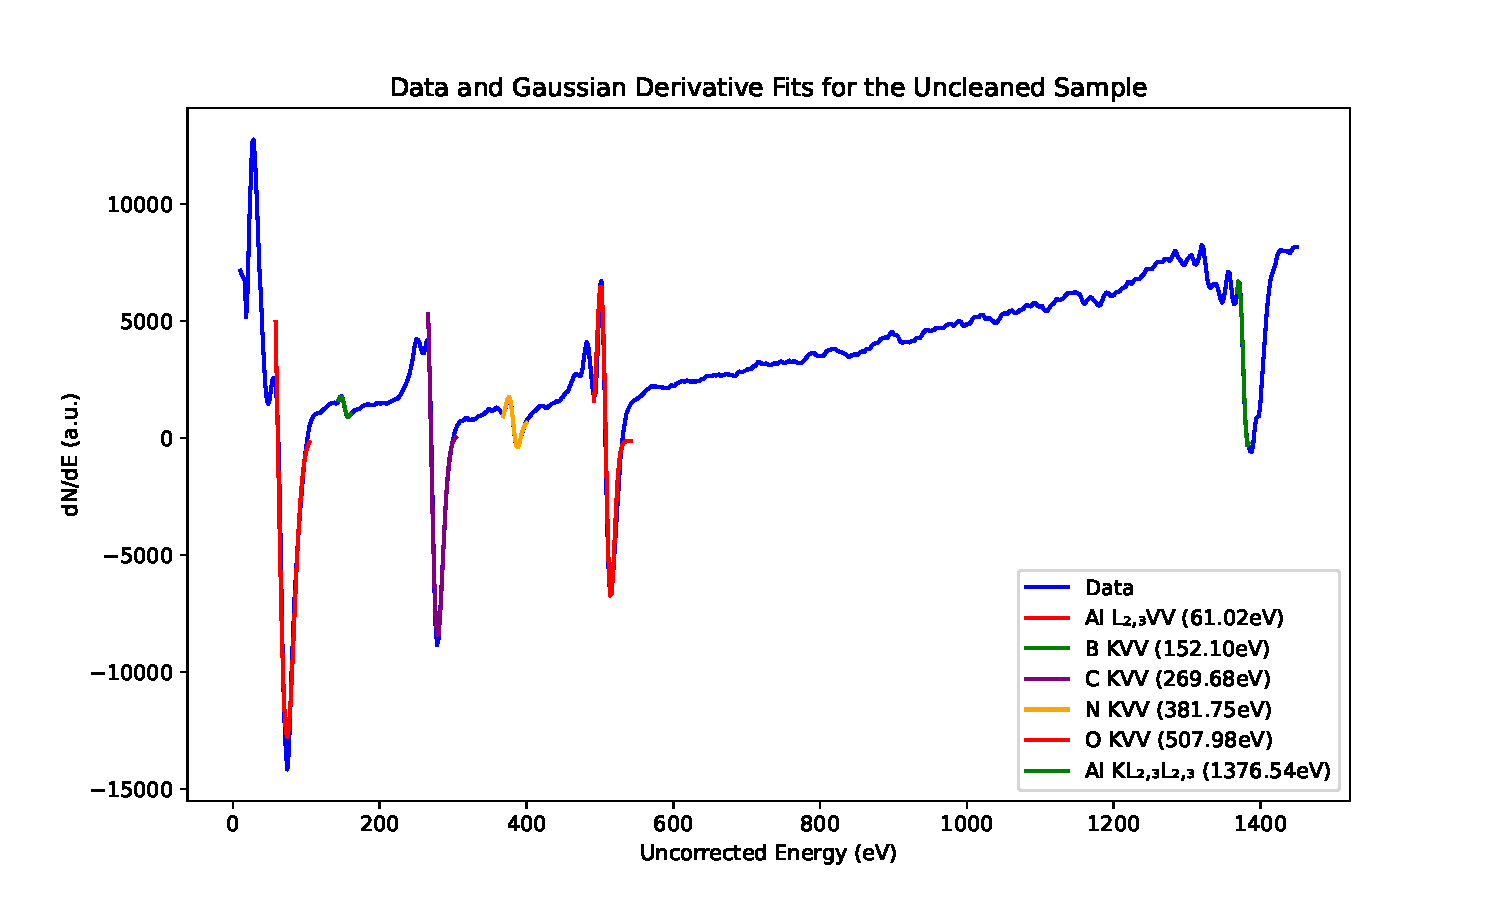
\includegraphics[width=\linewidth]{dirty.pdf}
  \caption{Full spectrum of the uncleaned Al sample, with Gaussian derivative fits.}
  \label{uncleaned}
\end{figure}

\begin{figure}
  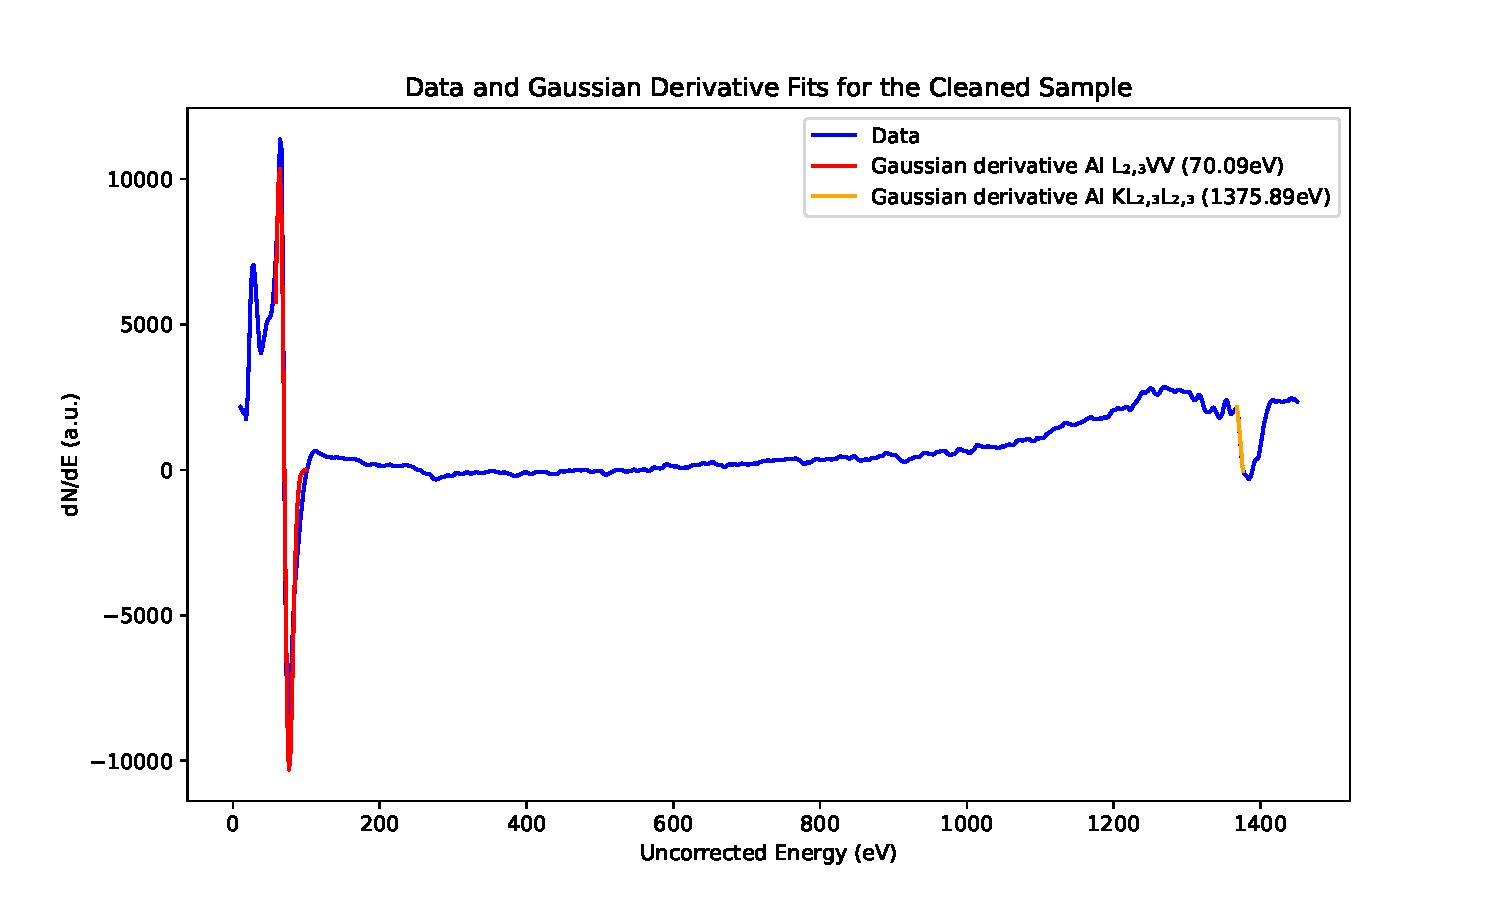
\includegraphics[width=\linewidth]{cleaned.pdf}
  \caption{Full spectrum of the cleaned Al sample, with Gaussian derivative fits.}
  \label{cleaned}
\end{figure}

\begin{figure}
  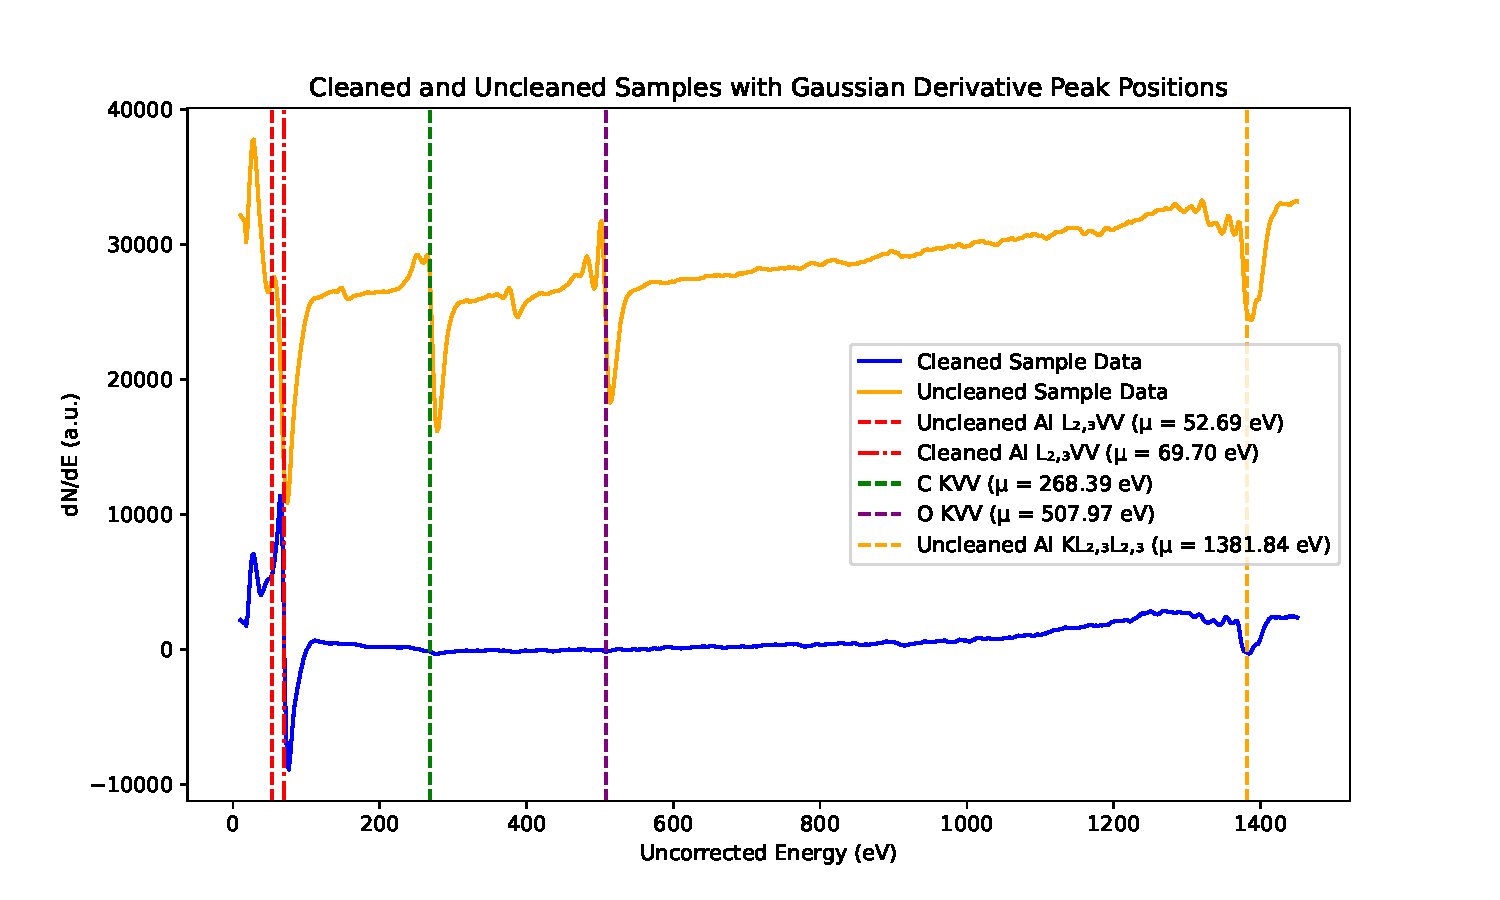
\includegraphics[width=\linewidth]{clean_dirty.pdf}
  \caption{Comparison of the uncleaned and cleaned Al Auger spectra.}
  \label{clean_dirty}
\end{figure}



\begin{table}[h!]
    \centering
    \begin{tabular}{lcccc}
        \toprule
        \textbf{Auger line} & \textbf{\(E_{\text{exp}}\) (eV)} & \textbf{\(E_{\text{uncorr}}\) (eV)} & \textbf{\(E_{\text{corr}}\) (eV)} & \textbf{\(E_{\text{lin}}\) (eV)} \\
        \midrule
        $\text{Al}_2\text{O}_3\text{/Al}$ $\text{L}_{2,3}$VV & 53.4 & 61.02 $\pm$ 0.50 & 77.98 $\pm$ 0.50 & 68.58 \\
        B KVV & 176.6 & 152.10 $\pm$ 0.12 & 169.06 $\pm$ 0.12 & 160.56 \\
        C KVV & 266.8 & 269.68 $\pm$ 0.22 & 286.64 $\pm$ 0.22 & 279.31 \\
        N KVV & 396.6 & 381.75 $\pm$ 0.08 & 398.71 $\pm$ 0.08 & 392.50 \\
        O KVV & 531.6 & 507.98 $\pm$ 0.24 & 524.94 $\pm$ 0.24 & 519.98 \\
        Al $\text{KL}_{2,3} \text{L}_{2,3}$ ($^{1}$D) & 1393.1 & 1376.54 $\pm$ 0.12 & 1393.50 $\pm$ 0.12 & 1397.17 \\
        \bottomrule
    \end{tabular}
    \caption{Comparison of expected (\(E_{\text{exp}}\)), uncorrected (\(E_{\text{uncorr}}\)), and corrected by moving the highest transition peak identified to 1393.5 eV (\(E_{\text{corr}}\)) energy values for Auger lines. Linear correction is provided as \(E_{\text{lin}}\). The uncertainties come from the Gaussian fits. The linear correction uses $a = 1.0099$ and  $b = 6.9501$. Check the Appendix for more details about the linear correction.}
    \label{tab:alpeaks}
\end{table}
\begin{table}[h!]
    \centering
    \begin{tabular}{lcccc}
        \toprule
        \textbf{Auger line} & \textbf{\(E_{\text{exp}}\) (eV)} & \textbf{\(E_{\text{uncorr}}\) (eV)} & \textbf{\(E_{\text{corr}}\) (eV)} & \textbf{\(E_{\text{lin}}\) (eV)} \\
        \midrule
        Al $\text{L}_{2,3}$VV & 67.2 & 70.09 $\pm$ 0.25 & 87.70 $\pm$ 0.25 & 67.20 \\
        Al $\text{KL}_{2,3} \text{L}_{2,3}$ ($^{1}$D) & 1393.1 & 1375.89 $\pm$ 0.34 & 1393.50 $\pm$ 0.34 & 1393.10 \\
        \bottomrule
    \end{tabular}
    \caption{Comparison of expected (\(E_{\text{exp}}\)), uncorrected (\(E_{\text{uncorr}}\)), corrected (\(E_{\text{corr}}\)) by shifting the last peak to 1393.5 eV, and linear correction (\(E_{\text{lin}}\)) energy values for Auger lines. The uncertainties come from the Gaussian fits. The linear fit correction uses the parameters $a = 1.0154$ and $b = 3.9689$.}
    \label{tab:alpeaksclean}
\end{table}

\subsection{Zoomed-in plot of the Al Auger Peaks (multiplet terms)}
For this task, it was necessary to first of all change the recording range to only focus on the KLL Al transiton - in our case from 1250 to 1450 eV. %todo this is very unspecific
Since the recording time was also suppressed, we changed the step size to 0.5 eV so as to get more data points.
Furthermore, the sensitivity was adjusted in order to maximize again the intensity of the greatest peak.
The parameters found to yield the best spectrum were a phase of 156\degree, a sensitivity of $100 \mu $V, a time constant of 300 ms, and the oscillator level of 1.5 V.
The recorded spectrum had its main peak at $1377.76\text{ eV}$, and was manually set to the theoretical value of $1393.5\text{ eV}$, which means that the correction shift is $15.74 \text{ eV}$ (Figure \ref{alzoom}). The resulting data was then compared to theory, leading to consistent results up to the experimental uncertainty (Table \ref{tab:transition_exp}).
%However, this was not enough to get a clear distinction of all the multiplett terms peaks: the

\begin{table}[h!]
    \centering
    \begin{tabular}{lccc}
        \toprule
        \textbf{Auger line} & \textbf{\(E_{\text{exp}}\) (eV)} & \textbf{\(E_{\text{uncorr}}\) (eV)} & \textbf{\(E_{\text{corr}}\) (eV)} \\
        \midrule
        K-L$_{2,3}$L$_{2,3}$ ($^{3}$P) & Not obs. & - & - \\
        K-L$_{2,3}$L$_{2,3}$ ($^{1}$D) & 1393.1 & 1377.76 $\pm$ 0.03 & 1393.50 $\pm$ 0.03 \\
        K-L$_{2,3}$L$_{2,3}$ ($^{1}$S) & 1387.1 & - & - \\
        K-L$_{2,3}$L$_{2,3}$ ($^{1}$D) + B1 & 1377.9 & 1361.82 $\pm$ 0.02 & 1377.55 $\pm$ 0.02 \\
        K-L$_{1}$L$_{2,3}$ ($^{3}$P) & 1357.2 & - & - \\
        K-L$_{1}$L$_{2,3}$ ($^{1}$P) & 1341.6 & 1326.66 $\pm$ 0.08 & 1342.39 $\pm$ 0.08 \\
        K-L$_{1}$L$_{2,3}$ ($^{1}$P) + B1 & 1326.4 & 1310.62 $\pm$ 0.26 & 1326.36 $\pm$ 0.26 \\
        K-L$_{1}$L$_{1}$ ($^{1}$S) & 1302.6 & - & - \\
        \bottomrule
    \end{tabular}
    \caption{Energy values for different Auger lines. Comparison of experimental values (\(E_{\text{exp}}\)), uncorrected (\(E_{\text{uncorr}}\)), and corrected (\(E_{\text{corr}}\)) by shifting the first peak to 1393.5 eV. The uncertainties for corrected energies come from the Gaussian fits. The $B1$ indicates bulk plasmon excitation, (the energy of a bulk plasmon was taken to be $15.2 \text{ eV}$, as stated in \cite{dufor}). Auger lines labeled "Not obs." and a dash were not visible in the spectrum.}
    \label{tab:transition_exp}
\end{table}
\subsection{Investigation of the plasmon-loss structure of aluminum}
\subsubsection{Bulk plasmons}
We then performed EELS bulk plasmon measurement. To do this, we set the acceleration voltage to around 1 keV, which according to the unversal mean free path diagram, is an energy sufficient to excite around 10 atomic layers below the surface. We recorded the spectrum from 960 eV to 1080 eV, with a phase of 156\degree, a sensitivity of $300 \mu $V, a time constant of 300 ms, and the oscillator level of 1.5 V.
Then we fitted gaussian derivatives to extrapolate the peak positions (Figure \ref{bulkplasmonss}).

Here, the excitation peak occurred at around 1041 eV (Table \ref{tab:mu_distances1}), and 3 other peaks to its left also were recorded, with each subsequent distance of $15 \pm 2 \text{ eV}$, which is consistent with the theoretical plasmon energy, within the fitting errors, which in this case were bigger. % which in this case is both due to the lock-in oscillator amplitude (1.5 V) and the resolution of 0.5 eV, and the fitting function.


\begin{table}[h!]
    \centering
    \begin{tabular}{lccc}
        \toprule
        \textbf{Plasmon} & \textbf{E (eV)} & \textbf{Peak Separation (eV)} \\
        \midrule
        B6          & $940.64 \pm 0.43$  & 16.93 $\pm$ 0.45 \\
        B5          & $957.57 \pm 0.14$  & 15.27 $\pm$ 0.16 \\
        B4          & $972.84 \pm 0.08$  & 14.93 $\pm$ 0.11 \\
        B3          & $987.77 \pm 0.08$  & 14.23 $\pm$ 0.11 \\
        B2          & $1002.00 \pm 0.07$ & 17.85 $\pm$ 0.08 \\
        B1          & $1019.85 \pm 0.04$ & 15.14 $\pm$ 0.06 \\
        Excitation  & $1034.99 \pm 0.05$ & -- \\
        \midrule
        \textbf{Average}  & --  & 15.73 $\pm$ 0.10 \\
        \bottomrule
    \end{tabular}
    \caption{Fitted parameters for bulk plasmons in the Al spectrum, with corresponding distances between consecutive peaks. The errors in energy (eV) are given for each peak, and the peak separations are shown with their uncertainties. The average peak separation is also shown with its corresponding uncertainty. We notice that the average separation is reasonably close to the theoretical value of 15.2 eV.}
    \label{tab:mu_distances1}
\end{table}

\subsubsection{Surface plasmons}
The acceleration voltage is now set at 200 eV, in order to excite only a few atomic layers below the surface. The spectrum was measured as before (same parameters), only in this case the sensitivity was decreased to $30 \mu $V, and the oscillation amplitude to 1.3 V to better resolve the peaks. Differently from before, fitting derivatives of Gaussian did not produce as good results as before, due to the spectrum being more noisy. Despite this, we still could identify the peak positions (Figure \ref{surfaceplasmonss}), and measure the distances between peaks, which are reported in Table \ref{tab:mu_distances2}.

The measurement error was taken to be the step size of 0.5 eV, and despite the imprecision, we were able to distinguish the surface plasmons (S1-4) from the bulk plasmons (B1-4) below the excitation energy level.

The presence of bulk plasmons in this case can be attributed to the relatively high excitation energy used in the experiment. When the excitation energy is elevated, the electrons possess enough energy to penetrate deeper into the material, which allows them to excite not only surface plasmons but also bulk plasmons that are generated within the bulk of the sample. The interaction of these energetic electrons with the sample results in the excitation of both types of plasmons. Reflecting on this, it is plausible that by lowering the filament energy even further, the electrons would have been less energetic, potentially preventing them from penetrating as deeply into the sample. This reduction in energy could have enhanced the ability to distinguish surface plasmons more clearly, as the excitation would have been more confined to the surface region, minimizing the contribution from bulk plasmons.
%There is also a rather big distance between B1 and B2 which may lead to believe that the CMA damage could also contribute to measurement errors. However, the distinction between surface and bulk can still be made, due to their energies of 10.5 and 15.2 eV respectively, which is resembled in our measurements within the uncertainty.


\begin{figure}[H]
  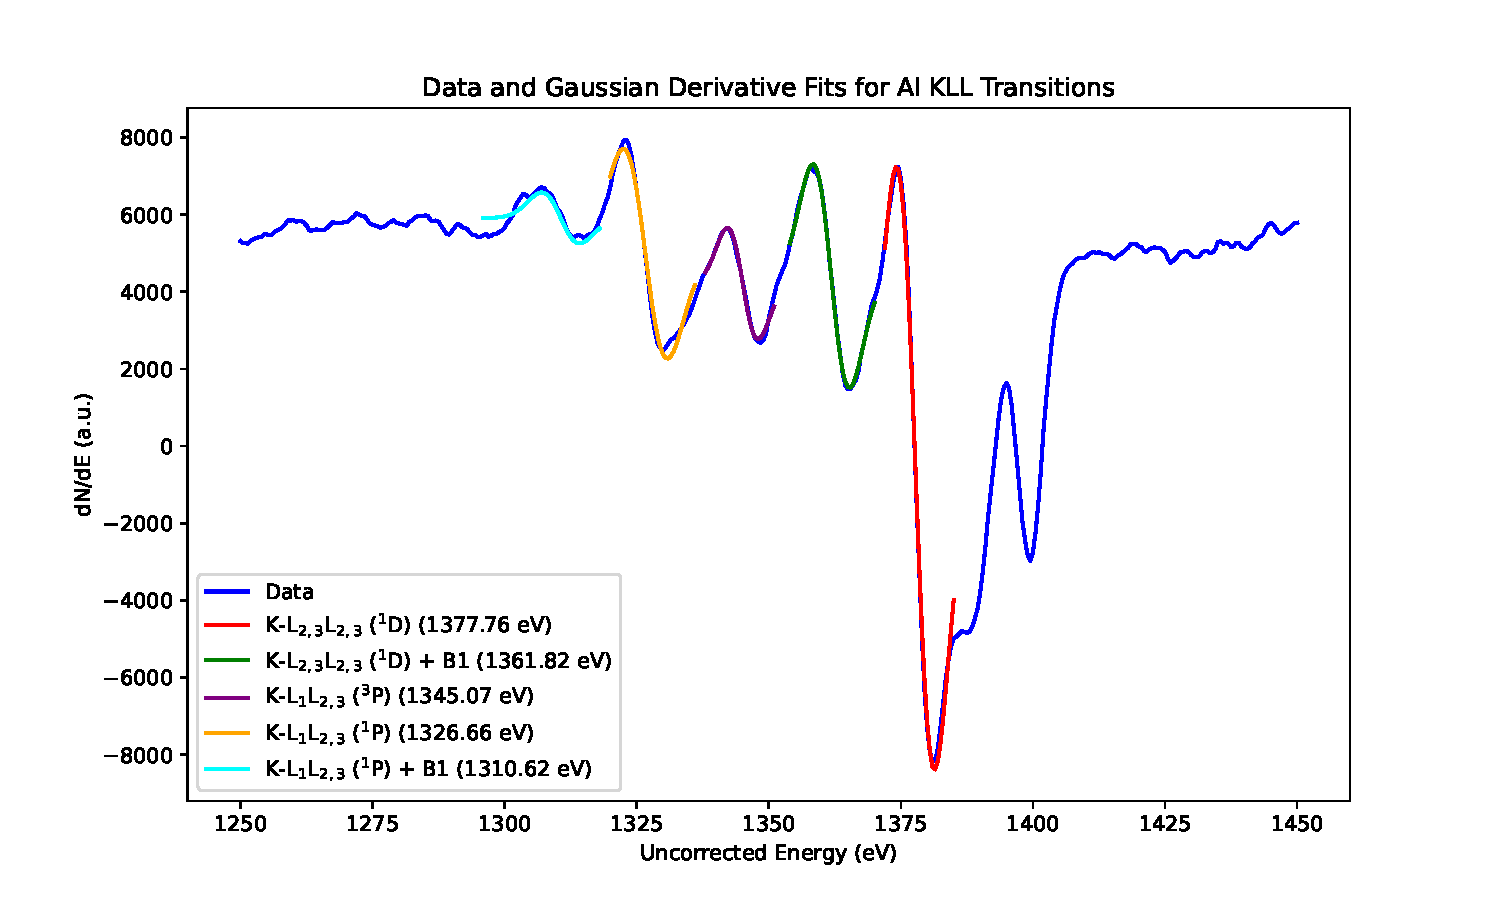
\includegraphics[scale = 0.49]{alzoom.pdf}
  \caption{Detail of the Auger KLL transition in Aluminum, with the respective fitting of the peaks. The obtained data is reported in Table \ref{tab:transition_exp}. It is to be noted here that the two peaks in the range 1400-1425 eV are due to damage in the detector and were thus not considered.}
  \label{alzoom}
\end{figure}

\begin{table}[H]
    \centering
    \begin{tabular}{lccc}
        \toprule
        \textbf{Plasmon} & \textbf{E (eV)} & \textbf{Peak Separation (eV)} \\
        \midrule
        Excitation  & $201.59 \pm 0.36$ & -- \\
        S1          & $194.05 \pm 0.02$ & $7.54 \pm 0.36$ \\
        B1+S1      & $186.02 \pm 0.02$ & $15.56 \pm 0.36$ \\
        B2          & $170.60 \pm 0.08$ & $15.42 \pm 0.08$ \\
        B3          & $154.21 \pm 0.26$ & $16.40 \pm 0.26$ \\
        B4          & $138.36 \pm 0.14$ & $15.84 \pm 0.14$ \\
        \bottomrule
    \end{tabular}
    \caption{Distances between consecutive plasmon peaks in the Al spectrum shown in Figure \ref{surfaceplasmonss}. We believe that only one peak (S1) is due to a surface plasmon excitation, as the energy distance from the Excitation peak is 7.54 eV which resembles the expected 10 eV. Then other peaks follow, but as their distance shows, they're probably due to bulk plamons. Furthermore the measurement was somewhat noisy, and thu sdistinction between surface and bulk plasmons may not be totally accurate, especially towards the lower energy region.}
    \label{tab:mu_distances2}
\end{table}






\begin{figure}[H]
  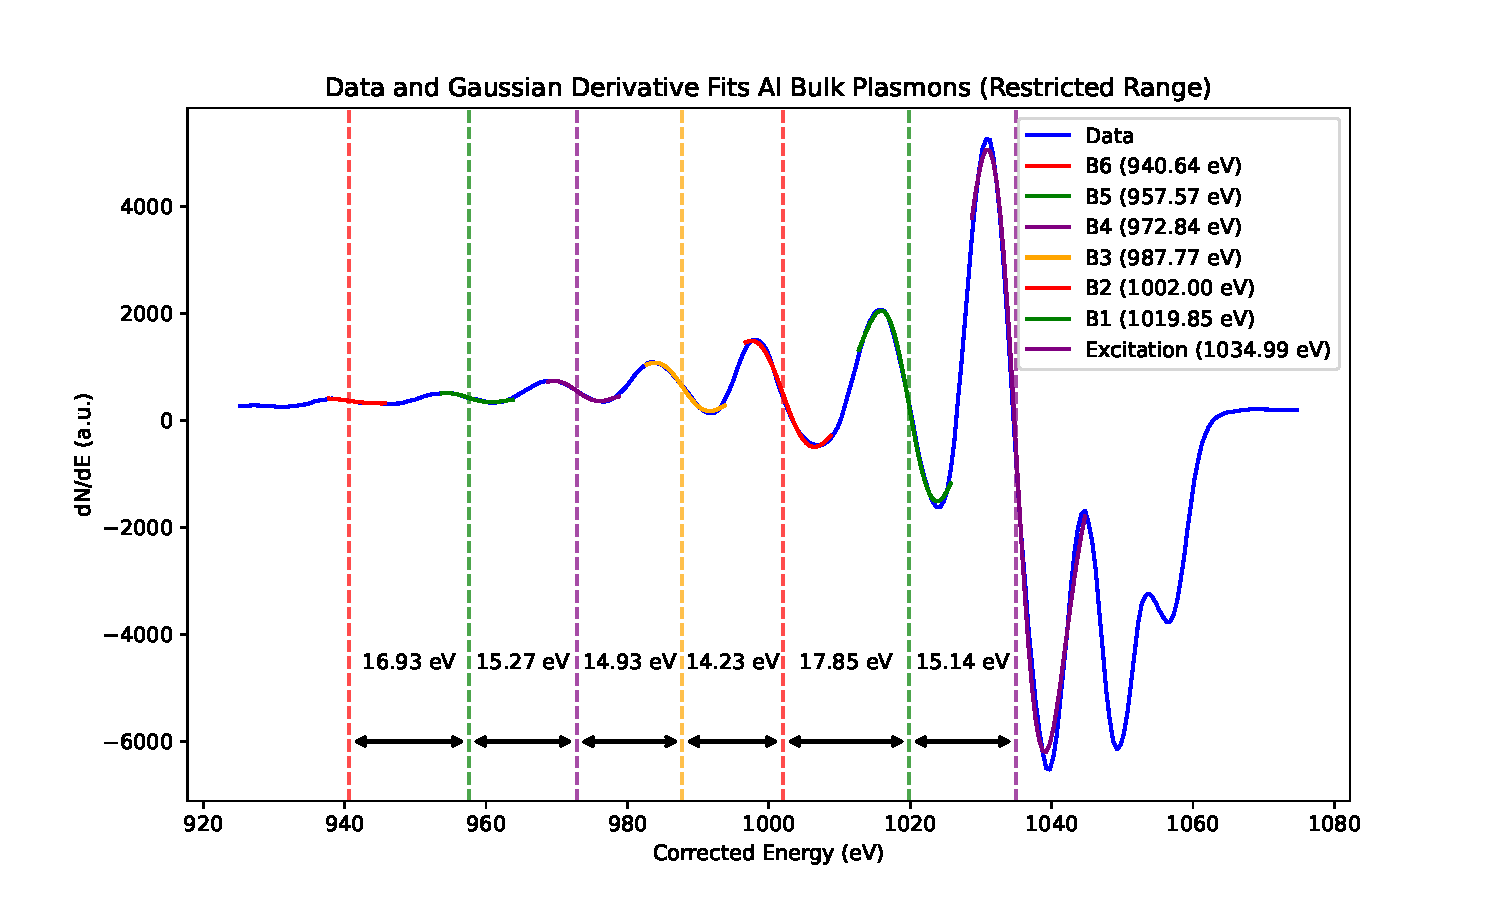
\includegraphics[scale = 0.49]{bulk.pdf}
  \caption{Bulk plasmon excitation for Al. Elastically scattered free electrons with energy of around 1keV create bulk plasmons with energy (15 ± 2) eV, which is consistent with the theoretical value of 15.2 eV \cite{dufor}. }
  \label{bulkplasmonss}
\end{figure}

\begin{figure}[H]
  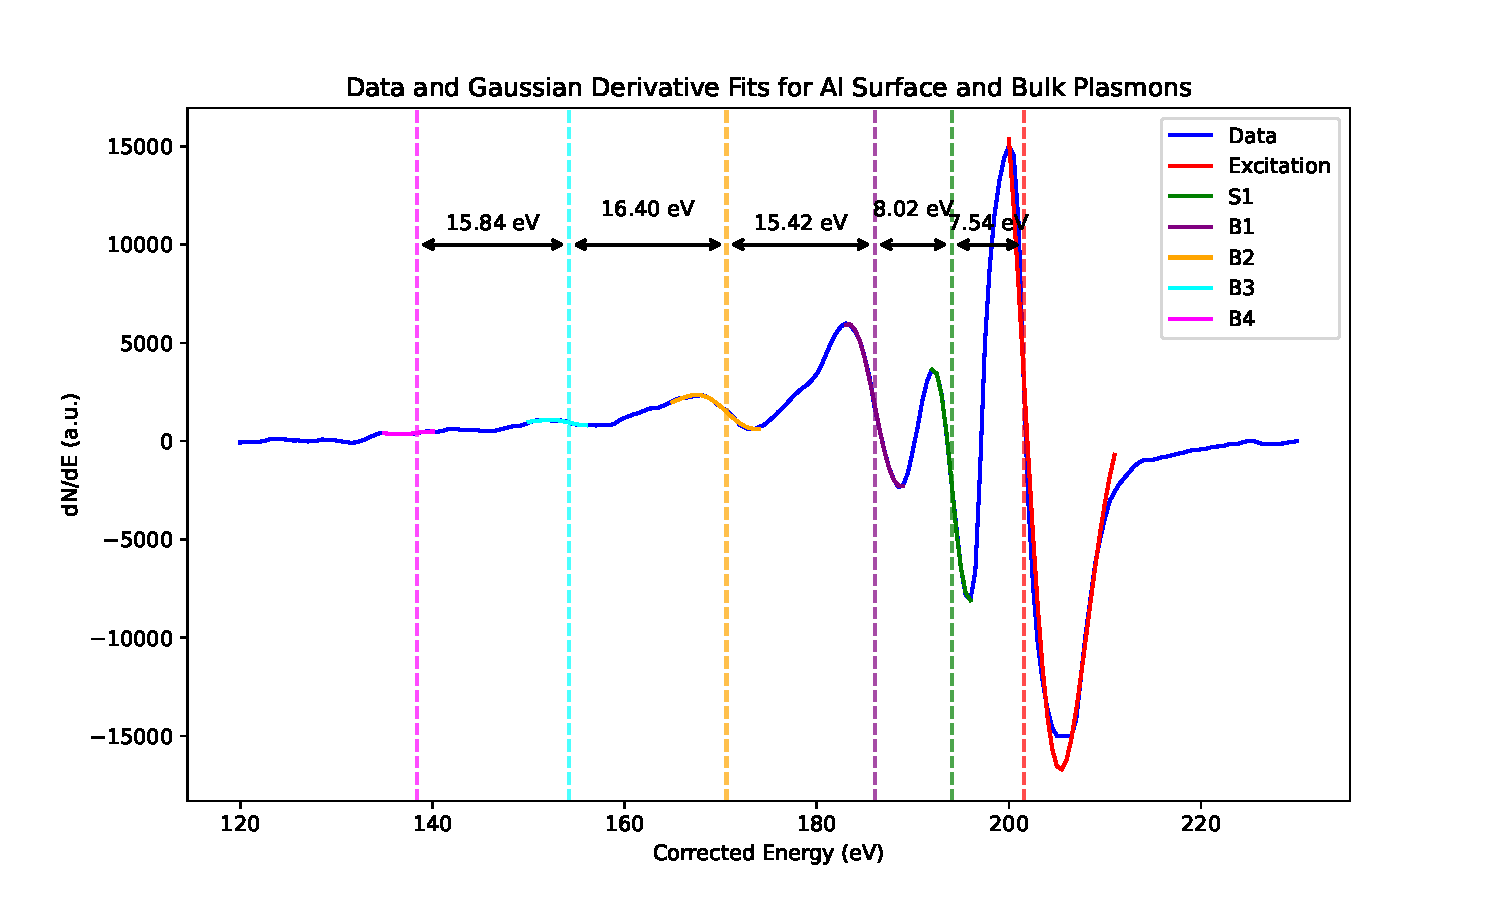
\includegraphics[scale = 0.49]{surfaceplasmons_30uV_156deg_300ms_1.9e-09mbar_200eV_Al_KLL_peaks_fit_with_baseline_plot_shifted.pdf}
  \caption{Surface plasmon excitation for Al. An energy of around 0.2 keV is used for the electrons that create the surface plasmon excitation. }
  \label{surfaceplasmonss}
\end{figure}


%However, there are two sources of error in our measurements: firstly, a sistematic error in the !!

\rule{\textwidth}{0.5pt}



\section{Summary and Outlook}
\rule{\textwidth}{0.5pt}

In this experiment, we investigated the Auger electron spectroscopy (AES) of uncleaned and cleaned aluminum samples. The uncleaned sample showed significant contributions from carbon and oxygen impurities, which were removed in the cleaned sample, resulting in a more intense Al $\text{L}_{2,3}$VV transition.

Additionally, our analysis of the Al Auger peaks revealed good agreement with theoretical values after correcting for instrumental shifts. The study of plasmon excitations showed clear evidence of bulk plasmon modes with energy losses around 15 eV, consistent with the expected value. Surface plasmons were also identified, with their energies significantly lower, at around 10 eV.

Future work could aim to improve experimental reproducibility and resolve minor discrepancies observed in the KLL transition and plasmon measurements by refining the experimental setup, particularly focusing on the CMA resolution and stability.

\section{Appendix: Linear correction}
To calibrate the energy values of the obtained Auger spectra, two methods were employed: shifting the value of the $\text{K}\text{L}_{\text{2,3}}\text{L}_{\text{2,3}}$ peak to the known expected energy (these values are denoted as $E_{corr}$ in our text; and a linear method ($E_{lin}$), which works similarly but uses the knowledge of other known peaks too.
The uncleaned spectrum (Figure \ref{uncleaned}) was used for the calibration. The way it was employed was to plot the NIST expected values of known peaks against what we obtained in the uncleaned spectrum. In particular, the KVV transitions for boron, carbon, nitrogen and oxygen, in addition to the Al LVV and KLL peaks. This resulted in the plot seen in Figure \ref{linear}. Then, linear fitting of the form $y = ax + b$ was used to obtain the energy values of the peaks that sit in this line and that generate the $E_{lin}$ values. The obtained $a$ and $b$ parameters are reported in the respective table descriptions.

This method gave slightly closer values to the expected ones, probably because it doesn't concentrate all its precision on one single peak, but it is spread along more peaks, which reduces the error.

\begin{figure}[H]
  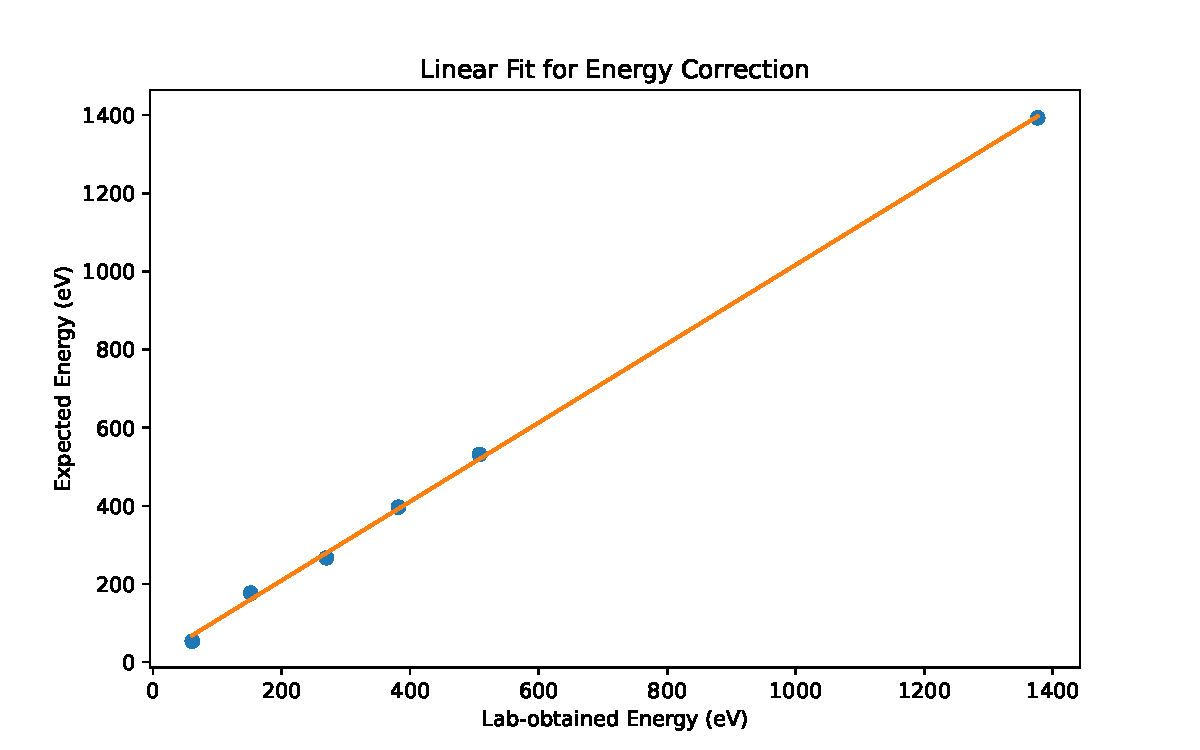
\includegraphics[scale = 0.7]{linear.pdf}
  \caption{Linear correction for the peak positions in the uncleaned sample. The peak positions correspond to those mentioned in Table \ref{tab:alpeaks} (from smallest to largest).}
  \label{linear}
\end{figure}
% Leave this section empty as per the request.
%\bibliographystyle{unsrt}
\printbibliography[heading=bibintoc]{}
\end{document}